\documentclass[a4paper,12,oneside,notitlepage]{report}
\usepackage[letterpaper, portrait, margin=2cm]{geometry}
\usepackage{listings}
\usepackage{url}
\usepackage{mhchem}
\usepackage{graphicx}
\usepackage{caption}
\usepackage{amsmath}
\usepackage{fancyhdr}
\usepackage{siunitx}
\usepackage{float}
\usepackage{epsfig,amsmath,amssymb,rotating,array}
\pagestyle{fancy}
\lhead{University of Sussex}
\rhead{Candidate No. 133884}
\renewcommand{\headrulewidth}{0.4pt}
\renewcommand{\footrulewidth}{0.4pt}
%\renewcommand{\section}[2]{}%
\renewcommand{\chapter}[2]{}%

\begin{document}
\title{Summer Research Placement Report: Supernovae Neutrinos}
\author{Michael Soughton, ms731@sussex.ac.uk \\
Supervisor: Simon Peeters,  \\
Working with: Bruno Zamorano}
\date{21$^{st}$ September, 2017}
\maketitle
\providecommand{\e}[1]{\ensuremath{\times 10^{#1}}}


\vspace{14cm}
\begin{abstract}
\noindent
\begin{center}
The Deep Underground Neutrino Experiment (DUNE), which is part of the The Long-Baseline Neutrino Facility (LBNF) currently under construction, aims to provide new information regarding the production of neutrinos inside supernovae. First, a reliable trigger for supernovae neutrinos must be made so that the full data-readout of a supernovae can be saved (full data steam is normally discarded). This project looked into obtaining useful Monte Carlo truth information of supernovae neutrinos which could be compared to background noise in order to produce a trigger. Initial findings show that hits from supernovae neutrinos occur within the detector in sufficiently different ways to background radiological noise such that the two sources could be decomposed to a good extent.
\end{center}
\end{abstract}

\newpage
\section*{\fontsize{11}{11}\selectfont Introduction }
During the last decade, the neutrino community has made efforts to construct a new generation of neutrino detectors. The Long-Baseline Neutrino Facility (LBNF) and the Deep Underground Neutrino Experiment (DUNE), due to be constructed in the next decade, will aim to have a 1.2 MW muon neutrino beam constructed at Fermilab by 2026 which will be upgraded to 2.4 MW by 2030. A near detector will detect neutrinos from the beam near it's source and the DUNE far detector will detect beam neutrinos and supernova neutrinos as well as other background neutrinos eight-hundred miles away and will consist of four 10 kt Liquid Argon Time Projection Chamber (LArTPC) modules located deep underground. DUNE will search for CP-violation in neutrino oscillations, determine the ordering of the neutrino masses, test the three-neutrino paradigm, search from proton decay if it exits and will provide new information on how supernovae explode \cite{LBNEVol1} and what new physics can be learnt from a supernova neutrino burst - there has only been one recorded supernova neutrino event. DUNE should be able to determine the time, flavour and energy structure of a neutrino burst, however in order to retrieve useful data from a neutrino burst, we must develop a trigger so that the data readout (4.6 Tb s$^{-1}$ from four 10 kt LArTPCs) will only be saved to memory in the event of a supernova. My project looked at investigating the properties of neutrinos and the resulting 'hits' within a detector from a supernova neutrino burst and what we will need to know to be able to trigger a supernova neutrino readout to aquire useful data should one occur. 
\vspace{0.5cm}

\section*{\fontsize{11}{11}\selectfont Supernovae Neutrinos, Liquid Argon Time Proportion Chambers (LArTPCs) and Monte Carlo (MC) Simulations }
Since my project would look into the detection of supernovae neutrinos, an understanding of the origin of these neutrinos and how they will be detected was required. Supernovae produce a very large number of neutrinos - around 99\% of their gravitational binding energy is converted into neutrinos. Supernovae are of two main types, type I and type II, each with sub-categories. Type I supernovae occur when a white dwarf - a lower mass star in its final evolutionary stage, which is prevented from collapsing from the pressure of electron degeneracy, accretes enough matter from another nearby star that the star becomes massive enough that it is favourable (it requires less energy) for electrons to be captured by protons that it does to fill electron states (electrons follow Fermi-Dirac statistics) and so neutrinos and neutrons are produced by electron capture as
$$e^- + p \rightarrow \nu_e + n$$
and the star starts to collapse until collapse is halted by stronger neutron degeneracy. The mass at which a white dwarf will collapse is always 1.44 Solar Masses (the Chandreska Limit). Type II supernovae occur when a supermassive star has reached the point in it's lifetime when it has converted a significant amount of its matter into heavier elements. Fusing elements heavier than iron is an endothermic process, so the star does not produce enough energy in the core to prevent collapse. In both cases, as the star undergoes core collapse, there are a large number of electrons and protons with enough energy to undergo inverse beta-decay/electron capture. This phase lasts for about 10 ms \cite{Scholberg}. As there is so much in-falling matter, many of the neutrinos interact with it, even though neutrinos cross-section is very small. The neutrinos that escape can be seen as an initial neutrino burst, which is when the detector must trigger a supernova. Most electron flavours are of electron neutrino, then of anti-electron neutrino with few (anti)-muon and (anti)-tau neutrinos.
\vspace{0.5cm}
\\It is thought that the interaction of these neutrinos with the in-falling matter is enough to prevent all the matter from falling into a black hole and to launch the matter outwards. After the accretion phase, there is the cooling phase as the clouds of matter expand outwards. We still see neutrinos on the order of 10 s, but the luminosity of all flavours will gradually decline. There will be minimal neutrino oscillations in the vacuum of space, although if the supernova occurs on the other side of the Earth to the detector, then there will be neutrino oscillations due to the Earth. The oscillations through the Earth are fairly well known down to a certain depth, although oscillations through the center will introduce uncertainty unless there is a detector on the other side of the Earth to give un-shifted results. 
\vspace{0.5cm}
\\A LArTCP is a large chamber mostly filled with Argon-40. Electron neutrinos will interact with the Argon-40 through inverse beta decay through the interaction
$$\nu_e + \ce{^{40}Ar} \rightarrow e^- +\ce{^{40}K^*} +m\gamma$$
where and $m$ is a positive integer (usually less than or equal to three). Similarly, anti neutrinos interact through
$$\bar{\nu_e}+\ce{^{40}Ar} \rightarrow e^+ + \ce{^{40}Cl^*}+m \gamma$$
LArTPCs only interact with supernova muon and tau neutrinos through NC (Neutral Current - a neutral $Z$ Boson mediates the interaction between neutrino and electron scattering)interactions as they do not have enough energy to produce a muon or a tau electron unlike the beam muon (and anti) neutrinos which have much more energy and so can interact through CC (Charged Current - a charged $W^+$ or $W^-$ Boson mediates a neutrino going to a lepton and a lepton going to a neutrino simultaneously) interactions.
\vspace{0.5cm}
\\The produced lepton travels off some trajectory with a high momentum, meaning that it ionises more Argon-40 along the way. An electric field (of strength 500 Vcm$^{-1}$) is applied across the TPC by an Anode Plane Assembly (APA) at one end and a cathode plane at the other \cite{LBNEVol4}. The ionised Argon will move towards the cathode plane and the electrons towards to APA. The APA consists of three planes of wires as shown in Figure \ref{fig:TPCFig1}. The U and V planes consist of induction wires which see a bipolar signal as an electron passes by. The Y plane consists of collection wires which see a unipolar signal as the electrons are collected on it. These three readings can be combined to determine the trajectory of the lepton and it's properties such as energy and momentum which can tell us about the neutrinos. However we must also know the time at which the interaction happens. The produced photons may move off to hit a photodetector, but there are not enough of them to signal that they were the products of the interaction. Fortunately, Liquid Argon is a good scintillator - the electrons from ionisation can recombine with an Argon nucleus which can then briefly bond with another before decaying, releasing more photons as the electrons are ionised again, which repeats until the electrons reach the APA plane or lose enough energy so that they cannot decay any further and remain bound to an atom. Enough photons are released to give a time for the interaction. Acrylic bars coated with Tetra-N-phenylbenzidine (TPB) or doped in bulk will be installed in the APA frame. Signals are then read out electronically to be used as a trigger for the interaction time in the Data Acquisition (DAQ). TPCs will be stacked back to back so that their APAs overlap. This will improve the chances of pile-up, where a large number of interactions occur within one event and physically close to each other in the detector meaning that there is an ambiguity to which interaction occurs before another one, but makes the construction more cost effective.
\begin{figure} [H]
\begin{center}
%\includegraphics[width=0.4\textwidth]{TPCFig1.png}
\caption{Figure showing the TPC and APA design. \cite{LBNETPCppt} \label{fig:TPCFig1}}
\end{center}
\end{figure}
\noindent The amount of neutrinos detected will depend on the supernovae type and distance from Earth. For a core-collapse event $\SI{10}{kPc}$ away from Earth, there will be of the order of a few hundred interactions per event (the smallest unit of time measured by the DAQ, which is $\SI{0.5}{\micro s}$) during the initial burst. This is orders of magnitude greater than the number of interactions from background sources, so would be immediately apparent when the DAQ is viewed. However the DAQ receives about $\SI{4.6}{Tb s^{-1}}$ of data which must be overwritten shortly after, meaning that important data such as a supernovae readout must be saved to memory. This is why we must construct a trigger which will know when a supernovae occurs and save the readout. To build this trigger, we must have information on some of the properties of supernovae neutrinos to be able to distinguish them from the background such as the number of interactions, their energy, momentum and many other properties of the interaction. Since real data will not be collected for a number of years, Monte Carlo (MC) simulations are used. MC simulations are a set of computational algorithms which give numerical results based on random sampling about a probability distribution. For example, say we expect the number of neutrino interactions (which we can call the number of MC truths - named truths since the simulation, these 'truths' are what are 'actually' happening) per event from a supernovae to be distributed according to a Poisson distribution.

\section*{\fontsize{11}{11}\selectfont Required software packages}
SNOwGLoBEs (Sudbury Neutrino Observatory General Long Baseline Experiment Simulator) is a software package (currently under development) which aims to simulate a supernova neutrino event occuring within a detector. SNOwGLoBEs computes the neutrino flux from a supernova under a given model of a supernova for a given flux model. The three models currently available are the Livermore model, the GVKM model and (most recently) the Garching model. The Garching model is the most relevant as it includes neutrino interactions within the supernova such as nucleon Bremsstrahlung, neutrino pair processes, weak magnetism and nucleon recoils, making it the best model of nuetrinos withing a supernova to date. After the flux has been calculated (and the resultant flux that an Earth-based detector 10 kpc from a supernova would recieve), SNOwGLoBEs then computes the cross-sections for interactions within a detector and uses smearing matricies to calculate the interaction product spectra and a detector response. Finally, detector efficiencies are calculated. 
\vspace{0.5cm}
\\SNOwGLoBEs required the software 'GLoBEs' to run. This can be downloaded from github and then using the \verb|'./configure'| followed by the commands \verb|'make'| and \verb|'make install'|, within the GLoBEs directory. However, one must ensure that the GSL (GNU Scientific Libraries) are included within the \verb|'PATH'| variable, otherwise one will have to specifiy when using \verb|'./configure'| the location of these libraries. SNOwGLoBEs can also be installed from github and installed in a similar fashion, although one must declare some environment variables to the GLoBEs installation files and to where SNOwGLoBEs is to be installed. One uses SNOwGLoBEs by generating .dat files containing flux information for a given model, compiling a 'pinched' file which is used to create the outputted .dat files whose data can be viewed using ROOT to produce histograms. More detailed instructions are available at \verb|'https://epp.phys.susx.ac.uk/SnoPlus/SuperNova/SnowGlobes'|.
\vspace{0.5cm}
\\ROOT is an object oriented framework for large scale data analysis, which utilises C++. It is capable of producing histrograms and other plots and has many in-built functions for optimising plots. A key feature of ROOT is that it utilises a data container called a tree, with its substructures branches and leaves, which are used to store data efficiently. ROOT has many depandancies, including gcc libraries. When attempting to run SNOwGLoBEs through ROOT on the local university run server, I had to ensure that the latest version of the gcc libraries were loaded in before sourcing ROOT.
\vspace{0.5cm}
\\The majority of my work on this project would be done on the Fermilab servers, thus one required a Fermilab account. One can make one following the instructions at \url{https://web.fnal.gov/collaboration/DUNE/SitePages/Getting%20Computer%20Accounts%20at%20Fermilab.aspx}. Since I already had an account, I renewed it for another year at \url{https://fermi.service-now.com/renew_acct_request.do}, although I also needed another password which can be done by calling \verb|9-00-630-840-2345|.
One will obtain their own directory on the Fermilab servers and the ability to access them. Fermilab uses Kerberos for strong authentication - one will have a kerberos pricipal and password. I would use this to login to the servers with the use of kinit. 
\vspace{0.5cm}
\\LArSoft (Liquid Argon Software) is a collaboration of software used which is used to simulate events within LArTPCs, which utilisies many libraries from ART (a collection of libraries useful for detectors). One can build a release of LArSOFT by following the instructions at \url{https://cdcvs.fnal.gov/redmine/projects/35ton/wiki/Getting_Started_Examples}, remembering to move to the feauture branch to be used (here 'feature/mbaird42/SupernovaAna') using \verb|git checkout|. When logging into a DUNE server, start-up scripts which source generic environment variables and commands used for LArSOFT, are automatically run. These can can be seen in my home directory \verb|'/dune/app/users/soughton'|. One may have to occasionally rebuild their LArSOFT release with a newer version following the same steps. One can build ones own code into the LArSoft repository using the \verb|'mrb i'| command. Once this is done, one can run their code over a file containing Monte Carlo truth and hit data using the 'fhicl' job file associated with ones code. For example I would run over a file using \verb|'lar -c supernovaana_job.fcl <filename>'|. This will output a .root file containing any histograms or N-Tuples created by the code which can then be viewed using ROOT.

\section*{\fontsize{11}{11}\selectfont Results from SNOwGLoBEs}
I assumed that supernovae neutrinos would follow the Garching flux model. This model was developed by running a Monte Carlo simulation to determine values for the average energies and fitting parameter $\alpha$ to produce flux values under the following relation
\begin{equation}
\phi(E_{\nu}) = N \left( \frac{E_{\nu}}{<E_{\nu}>} \right)^\alpha \exp \left( -(\alpha + 1) \frac{E_{\nu}}{<E_{\nu}>} \right),
\end{equation}•
\\where $N$ is a normalisation constant. Under the Garching model, SNOwGLoBEs was used to produce a time evolution plot in terms of neutrino luminosoity, average energy and $\alpha$ as seen in Figure  \ref{fig:SnowglobesPlot1}. This plot reaffirmed what was expected about the energies and the events per bin for a supernova event and so I could proceed with the knowledge of what charachteristics a trigger should look for.
\begin{figure} [H]
\begin{center}
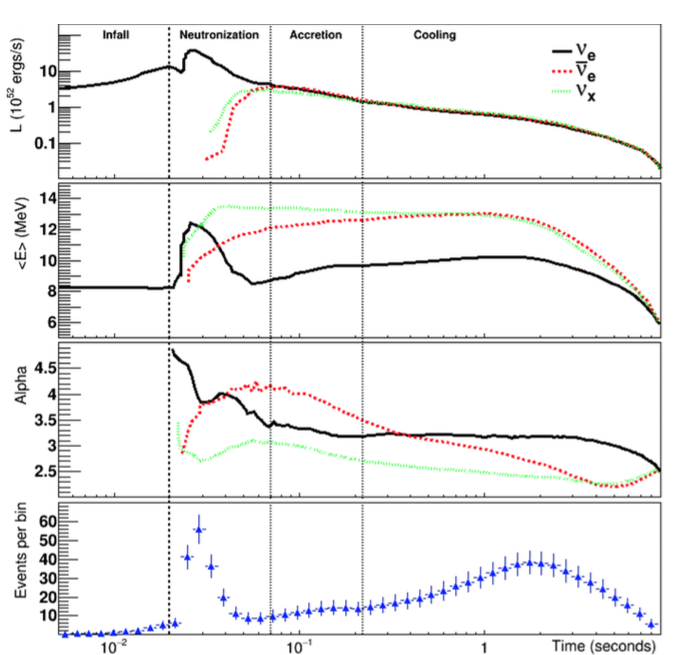
\includegraphics[width=0.4\textwidth]{SnowglobesPlot1.png}
\caption{Figure showing the time evolution of a supernova under the Garching model.  \label{fig:SnowglobesPlot1}}
\end{center}
\end{figure}


\section*{\fontsize{11}{11}\selectfont Investigation of hits within the detector}
My work would focus on finding a correlation between the positions of reconstructed hits within the detector from a supernovae event. I continued to edit my supernova analyser module code that I was working on in the summer of 2016. The module gets truth and hit information from the event and then fills an N-Tuple. Once having built and updated version of this code into the LArSoft repository I was using, I could run this analyser code over files containing truth and hit information for supernova neutrinos and their products, background radiological noise and electrical noise or any combination thereof. 
\vspace{0.5cm}
I needed to obtain information on the hits within the dector. A hit is counted as when an electron hits the APA plane, but its location and time is reconstructed to be where the electron is initially created - where it was ionised from an atom or the location of the neutrino interaction for the original lepton. One issue which appeared was that a frequency histogram of the $x$-position of hits (the electrons drift in the $x$ direction towards the APA) shows a Gaussian-like, but non-Gaussian distribution of electrons as seen in FIGURE X, whilst the histograms for the $y$ and $z$ hit positions were uniformly distributed. It was hypothesised that this was due electrons losing energy as they drift towards the APA and so any electrons which lose enough energy permantly re-ionise and as not seen as hits. To test this hypothesis...


\section*{\fontsize{11}{11}\selectfont Finding hit problems}
From the plots of detector angle vs number of hits and of detector angle vs summed ADC, for the file with only one neutrino, it was apparent that there were some events for which no hits or ADC was recorded, although all the other truth information was properly loaded. This implied that the simulation was failing to simulate events correctly the detector geometry. We initially wanted to see if electrons could be hitting the APA frame so would not count as a hit or give any ADC signal. To investigate this, I added the initial $x$,$y$,$z$ and $t$ information for the electrons (there would be negligible drift) and made plots of the vertices FIG. If electrons were hitting the frame, then with a cut for number of hits equal to zero, would just show the where electrons had hit the frame. This was not the case however, the hits still appeared randomly distributed with the cut. Michael produced some more supernova file, containing a larger number of events. These files had the same problem of getting zero hits or summed ADC. I had to update my release of LArSOFT following the steps as before and change some of my header files to match during this time as the new files depended upon the new release. I constructed numerous plots in attempt to uncover why this problem was occurring. A plot of the number of particles involved in the interaction (normally an electron neutrino, and electron and a few photons) against time revealled that some particles around $t=0$ did not have any hits. A plot of $x$ (the electrons drift in the $x$ direction towards the APA) against $t$ shown in Figure \ref{fig:xVtHisto} revealed why. About half the events occurred too far away and too late for the electrons to drift to the APA by the end of the simulation window. This demonstrated a problem with the simulation times, not with the physics involved and could be rectified by stopping events at a certain time and keeping the simulation running for long enough for the electron to reach the APA, although this would require more CPU, it should not be a problem for actual data as the readout is continuous. Still, this had uncovered a problem which would be a major hindrance in using MC data to build a working supernova trigger. With this solved and all the MC data, we can now look into building the trigger, which will need to compare the properties of a supernova burst to the background and determine when to start saving data. This will take time but is now achievable.
\begin{figure} [H]
\begin{center}
%\includegraphics[width=0.8\textwidth]{xVtHisto.png}
\caption{Histogram of initial $x$ position against initial $t$ of electrons with cuts. \label{fig:xVtHisto}}
\end{center}
\end{figure}

\section*{\fontsize{11}{11}\selectfont Summary}
During my project gained further experiance in the programs and software I was be using. I also had to read-up on Liquid Argon detectors and supernovae neutrinos. I managed to write code in C++ which would get useful Monte Carlo truth and hit information about a neutrino interaction and produce histograms with the information which will be useful in distinguishing the difference between supernovae neutrinos and background noise.  

\newpage
\section*{\fontsize{11}{11}\selectfont My Experiences}
I thoroughly enjoyed working on this project. My understanding of particle physics and of how experiments work has improved greatly. I have also gained experience of working with C++, SNOwGLoBEs, ROOT, LArSOFT and ART and of being in a real research group. I found the project to be challenging, but I liked that aspect as I was able to solve problems that I would not have otherwise faced during my studies.

\section*{\fontsize{11}{11}\selectfont Biography}
I have just completed my third year at Sussex, on the MPhys with Research Placement course. In the future, I would like to obtain a PhD and pursue a career in research. My areas of interest are particle physics and early-universe cosmology.


\newpage
\section*{\fontsize{11}{11}\selectfont Bibliography}
\begin{thebibliography}{20}

\bibitem{LBNEVol1} 
	R. Acciarri \textit{et at.} (2016),
	\emph{Long-Baseline Neutrino Facility (LBNF) and
Deep Underground Neutrino Experiment (DUNE)}.
	arXiv:1601.05471
		 
\bibitem{Scholberg} 
	K.Scholberg (2012),
	\emph{Supernova Neutrino Detection}.
	Department of Physics, 
	Duke University, Durham NC 27708, USA,
	
\bibitem{LBNEVol4} 
	R. Acciarri \textit{et at.} (2016),
	\emph{Annex 4A: The LBNE Design for a Deep
Underground Single-Phase Liquid Argon TPC}.
	 arXiv:1601.02984
	
\bibitem{LBNETPCppt} 
	B.Viren,
	\emph{Wire Cell Event Reconstruction Software
for LArTPC Detectors}.
	PowerPoint Presentation,
	Department of Physics,
	Brookhaven National Laboratory,
	2015	

\end{thebibliography}

\end{document}
